


\subsection{架構設計}

我們參考了 Clean architecture 與 MVVM 來設計架構,引入依賴反轉、雙向數據綁定等特性,旨在減少模組之間的依賴與增加可重用性,使得各部分能獨立開發和測試,並使得未來對系統的修改和擴展更為容易。此外,明確的架構和分層可以幫助團隊成員更快地瞭解專案結構,並減少彼此之間的工作衝突。

我們定義了兩種資料容器:

\begin{enumerate}
    \item Entity:作為系統中的主要資料容器,包含旅程、軌跡、座標點等核心資料。
    \item QueryItem:向外部資料庫(如SQL)請求數據獲得的原始結果,格式與資料表的定義相同。
\end{enumerate}

\begin{figure}[H]
    \centering
    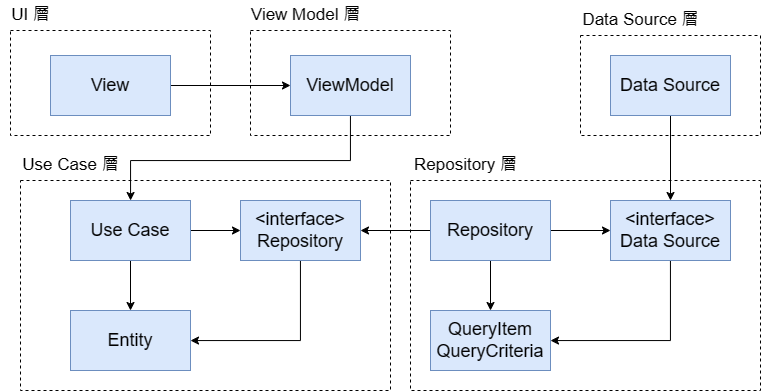
\includegraphics[width=0.8\textwidth]{assets/TT分層依賴圖.png}
    \caption{分層依賴圖}
    \label{分層依賴圖}
\end{figure}

我們將系統架構分為 Use Case、Repository、Data Source、View Model 和 UI 五層,圖~\ref{分層依賴圖} 為分層依賴圖,展示了各層內部的元件與依賴關係,以下將對各層進行詳細說明。

\begin{enumerate}

    \item Use Case 層:

    負責業務邏輯的處理,使用 Entity 作為資料容器。當 View Model 發起請求時,Use Case 會根據需求,調用 Repository 來獲得或操作數據。該層也定義了抽象的 Repository 介面。

    \item Repository 層:

    實作 Use Case 層定義的介面,負責從 Data Source 調用數據,取得 QueryItem 後轉換成 Entity 格式回傳給 Use Case。該層也定義了抽象的 Data Source 介面。

    \item Data Source 層:

    負責實際的數據存取。根據 Repository 的請求,Data Source 會去操作實際的數據來源,如資料庫、遠端服務或記憶體暫存等等,並以 QueryItem 作為回傳結果。

    \item View Model 層:

    該層為 MVVM 架構中的一部分,透過 Flutter 的 ChangeNotifier 實作。負責管理 UI 所需的狀態和邏輯。它會和 UI 進行雙向數據綁定,並透過 Use Case 處理業務邏輯和數據操作。

    \item UI 層:

    主要負責呈現使用者界面與互動。所有的 UI 元件都在這一層並組合成頁面,再透過 View Model 來獲得及顯示必要的數據。

\end{enumerate}
